\section{Baseline Design Validation and Projected Photon Detector Performance}
\label{sec:dp-pds-performance}

Subsequent to our initial simulation studies described in the \dshort{tp} \cite{Abi:2018rgm}, much progress has been made to advance towards a more realistic understanding of the projected \dshort{pds} performance using the \dshort{larsoft} framework:
%
\begin{itemize}
\item Optical simulations are now performed in the \dword{dp} \dword{fd} module geometry. In the \dword{fd} \dshort{tp}, physics studies assumed the \dword{pddp} geometry. Considering the lack of any optical segmentation in the \dword{dp} design, light is simulated in the full \dpactivelarmass \dshort{tpc} active volume. Simulation assumptions for light generation and light transport are described in Sec.~\ref{subsec:dp-pds-simulation_assumptions}. For each one of the \dpnumpmtch \dwords{pmt}, simulations take into account how the photon detection probabilities and the photon propagation times vary throughout the \dshort{tpc} active volume.
%
\item The simulation of the electronics response, as well as the reconstruction of optical hits and optical clusters, is now accounted for. Simulation assumptions for light detection by the \dwords{pmt} are also described in Sec.~\ref{subsec:dp-pds-simulation_assumptions}. Optical hits are the reconstructed optical signals on single \dshort{pmt} waveforms, and are characterized by a hit time, amplitude, and charge. Optical hits are required to have an amplitude of at least \SI{10}{ADC counts} above baseline. Optical clusters refer to a collection of \dshort{pmt} hits that are correlated in time and space. They are typically induced by the same underlying flash of scintillation light in \lar. The parameters of the clustering algorithm are discussed later in this section.

\fixme{Need to repeat the studies for a \SI{15.4}{\ns} sampling and a correspondingly reduced S/N ratio (latter number TBD, check with Antonio).}

%
\item The physics studies now also include radiological backgrounds. The simulation of radiological backgrounds is critical in order to perform a realistic optimization of the optical reconstruction parameters. The radiological model includes several radio-isotopes throughout the \lar volume, with \SI{1.01}{\becquerel/\kg} of $^{39}$Ar providing the largest activity. In addition, an impinging neutron flux of \SI{e-5}{\cm$^{-2}$\s$^{-1}$} is accounted for.
\end{itemize} 

\fixme{Need to check that neutron component of radiological model is implemented correctly}

Expected \dword{pds} light yields in the \dword{pddp} and \dword{dp} \dword{fd} module geometries are discussed in Sec.~\ref{subsec:dp-pds-simulation_yields}

%%%%%%%%%%%%%%%%%%%%%%%%%%%%%%%%%%%%%%%%%%%%%%%%%%%%%%%%%%%%%%%%%%%%

\subsection{Event $t_{0}$ Reconstruction}
\label{subsec:dp-pds-performance_t0}

As discussed in Sec.~\ref{sec:dp-pds-requirements}, event $t_0$ reconstruction for non-beam events via the \dshort{pds} is particularly important in order to be able to fiducialize nucleon decay candidates in \dword{dune}. Proton decay signal events with a %\ptoknubar 
$p\rightarrow K^{+} \bar\nu$ final state have been simulated with GENIE \cite{Andreopoulos:2009rq} throughout the \dword{dp} \dshort{tpc} active volume, and their optical clusters were reconstructed according to the simulation and reconstruction chain described above. NDK events are expected to deposit about \SI{400}{\MeV} visible energy in the \lar. The same reconstruction algorithm has also been applied to the simulated radiological backgrounds. In a first cluster reconstruction step, three parameters are optimized, in order to group optical hits into separate clusters:
%
\begin{description}
\item[Maximum cluster duration:] maximum time difference between all \dshort{pmt} hits in the cluster.
\item[Maximum hit time distance:] maximum time difference between successive \dshort{pmt} hits in the cluster. By definition, this quantity is smaller than the maximum cluster duration.
\item[Maximum hit distance:] maximum spatial distance between neighbouring \dshort{pmt} hits in the cluster. 
\end{description}
%
\begin{dunefigure}[Optimization of optical cluster parameters for NDK events.]{fig:dppd_ndk_optimization}
     {Optimization of optical cluster parameters for NDK events. For a \SI{1}{\us} maximum cluster duration, a maximum efficiency of NDK clusters above a minimum charge threshold is achieved for an \SI{800}{\ns} maximum hit time distance and a \SI{2.5}{\m} maximum hit distance.}
    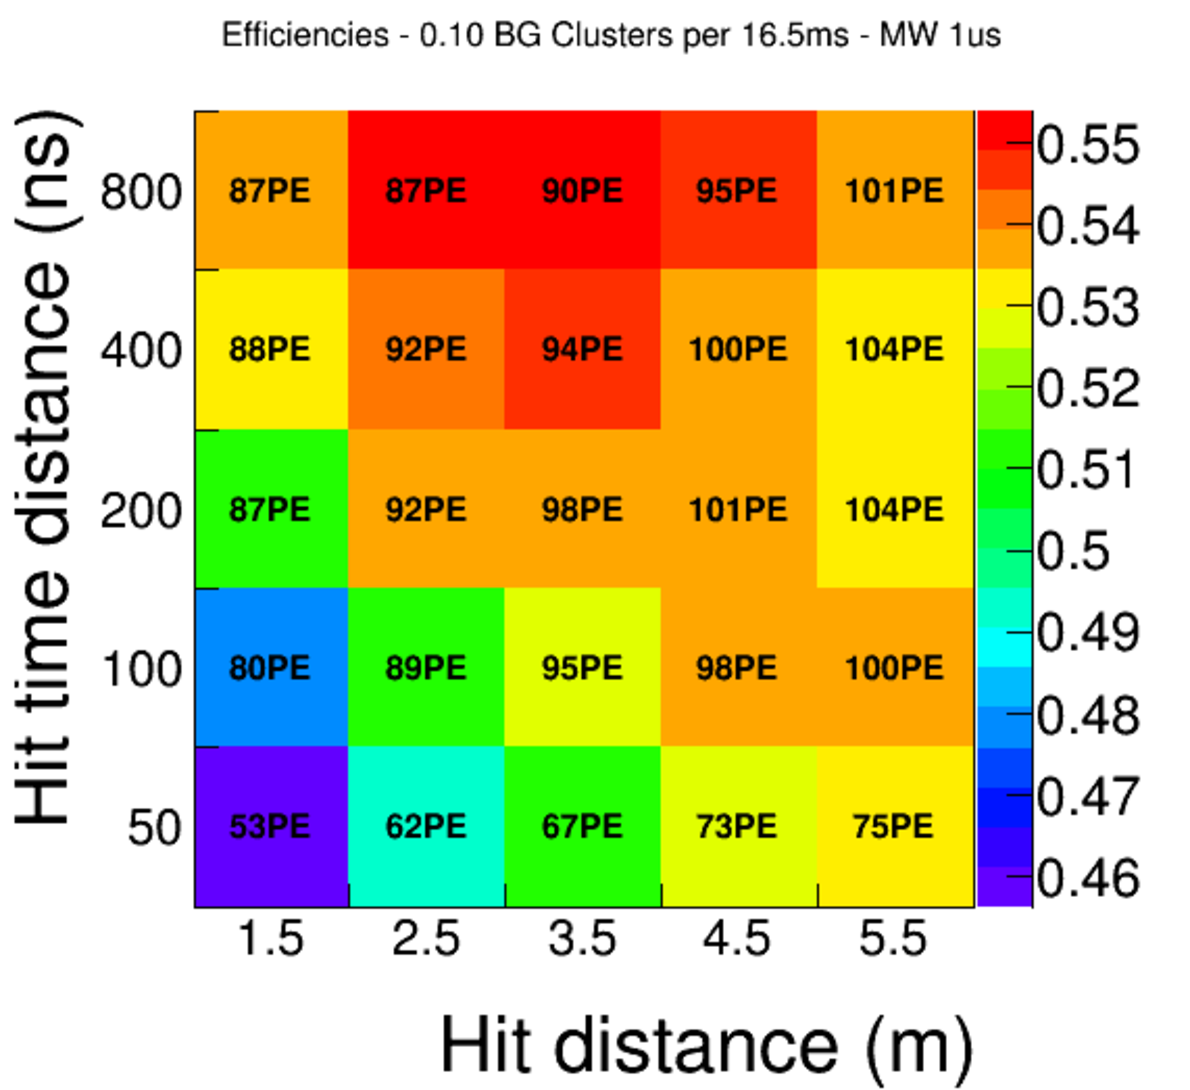
\includegraphics[width=0.5\textwidth]{graphics/dppd_ndk_optimization.pdf}
    \end{dunefigure}

For each chosen set of (maximum cluster duration, maximum hit time distance, maximum hit distance) parameters, a threshold on minimum cluster charge (in PEs) is defined, such that a fixed, and tolerable, radiological background rate of 0.05 clusters above threshold and per \SI{7.5}{\milli\s} maximum drift time is obtained. The chosen parameters are the ones that maximize the efficiency of detecting a NDK cluster above this minimum cluster charge. Figure~\ref{fig:dppd_ndk_optimization} illustrates the optimization process of the maximum hit time distance and maximum hit distance parameters for NDK events. As shown in the figure, the optimal values of the maximum hit time distance and of the maximum hit distance were found to be \SI{800}{\ns} and \SI{2.5}{\m}, respectively. Recalling that the \dwords{pmt} are located on a square lattice with \SI{1.02}{\m} pitch, a \SI{2.5}{\m} maximum hit distance means that the cluster can contain gaps in its hit pattern along a single \dshort{pmt} row or column. The maximum cluster duration was optimized in the same way, and set to a value of \SI{1}{\us}.

After clustering optical hits as described above, and without applying any threshold on cluster charge, several optical clusters per event are reconstructed. At this stage, any deposit resulting in at least one optical hit is reconstructed by the \dshort{pds}, resulting in negligible NDK optical cluster inefficiency but very high radiological background cluster multiplicity per event. In a second optimization step, we define the $t_0$ candidate clusters in the event as the ones fulfilling one additional condition:
\begin{description}
\item[Cluster spatial position:] albeit much less accurate than the \dshort{tpc} one, the \dshort{pds} response also provides some spatial information of the event in the plane perpendicular to the drift direction. We require the position of the $t_0$ candidate cluster in the plane perpendicular to the drift to be within \SI{2.5}{\m} of the simulated NDK decay vertex\footnote{The matching in position with the MC truth information is of course only possible in simulations. However, we expect the \dshort{tpc} imaging performance to be so superior with respect to the \dshort{pds} one that matching \dshort{pds} position with MC truth position is essentially equivalent to matching \dshort{pds} position with \dshort{tpc} reconstructed position.}. Since radiological clusters are randomly distributed with respect to the NDK vertex, this matching in position provides background cluster suppression.
\end{description}

We define the {\bf NDK $t_0$ reconstruction efficiency} as the efficiency to reconstruct at least one $t_0$ candidate cluster associated to the NDK energy deposit. As shown below, the cluster spatial position requirement causes some inefficiency for events farther away from the \dshort{pds}, because of poorly reconstructed cluster spatial position in the plane perpendicular to the drift.

In general, several $t_0$ candidate clusters will be reconstructed per event, induced by the NDK signal, by radiological activity and by \dshort{pmt} dark counts. If more than one choice exists, event $t_0$ information is associated to the $t_0$ candidate cluster of highest charge. For events where at least one $t_0$ candidate cluster exists, we define the {\bf NDK $t_0$ reconstruction purity} as the probability for the highest charge $t_0$ candidate cluster in the event to be associated with the NDK signal. A purity value $<1$ can be obtained if the highest charge $t_0$ candidate cluster is due to radiological activity. The choice of choosing the $t_0$ candidate cluster of highest charge is made to maximize the purity, since radiological clusters have fewer reconstructed PEs per cluster, on average. As discussed in Sec.~\ref{sec:dp-pds-requirements}, we require a high purity to minimise $t_0$ reconstruction ambiguities.
%

\begin{dunefigure}[Optimization of $t_0$ candidate cluster spatial position reconstruction for NDK events.]{fig:dppd_ndk_optimization2}
{Efficiency, purity and efficiency times purity for the $t_0$ candidate cluster to be correctly associated to the NDK energy deposit, as a function of the maximum 2D distance between the \dshort{pds}-reconstructed position of the $t_0$ candidate cluster and the actual NDK vertex, in the plane perpendicular to drift. A maximum distance of \SI{2.5}{\m} is the one that optimizes the product of efficiency times purity.}
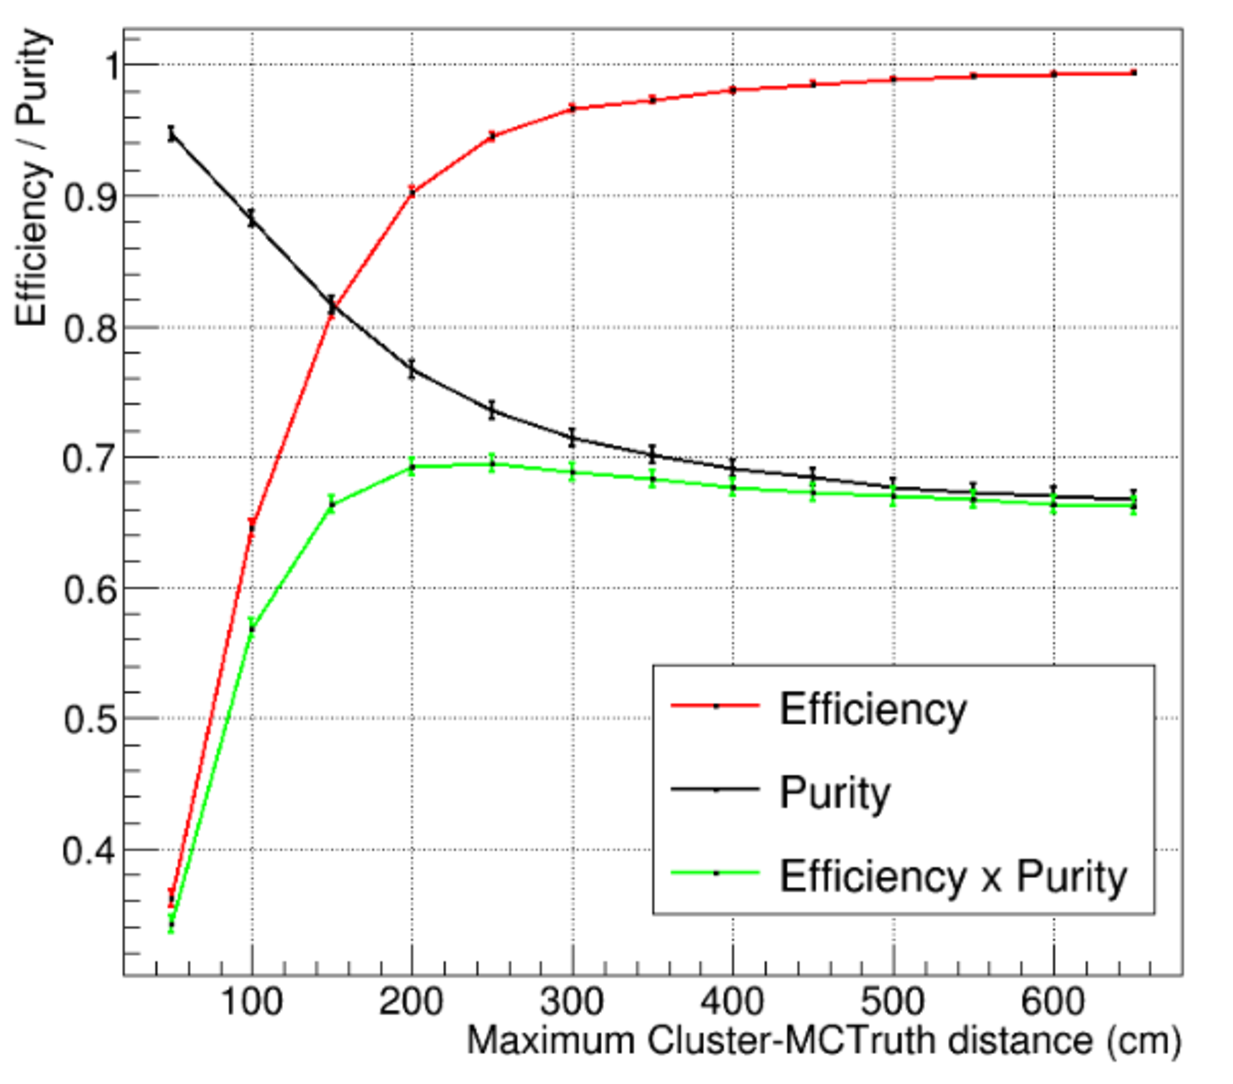
\includegraphics[width=0.5\textwidth]{graphics/dppd_ndk_optimization2.pdf}
\end{dunefigure}

Figure~\ref{fig:dppd_ndk_optimization2} illustrates how the NDK signal efficiency, purity, and efficiency$\times$purity averaged over the entire \dshort{tpc} active volume vary as a function of the 2D distance between the $t_0$ candidate cluster reconstructed position and the NDK vertex actual position, in the plane perpendicular to drift. A maximum distance of \SI{2.5}{\m} is the one that optimizes the product of efficiency times purity. For this optimal distance, average efficiency and purity values of \num{95}\% and \num{73}\%, respectively, are obtained.  

Figure~\ref{fig:dppd_ndk_efficiency} shows how the NDK $t_0$ reconstruction efficiency and purity vary as a function of the nucleon decay vertex distance from the cathode plane, for the optimal cluster reconstruciton parameters described above. As can be seen, the efficiency (purity) remains $>90\%$ for distances up to \SI{10}{\m} (\SI{7}{\m}) from the cathode. However, both quantities drop rapidly at large distances from the cathode, resulting in the 95\% and 73\% average quantities quoted above. This drop in efficiency and (especially) purity is caused by the marked reduction in the detected NDK light yield as the energy deposition occurs at increasingly larger distances from the cathode, see Fig.~\ref{fig:dppd_fd_light_yield_comparison}. From this figure, a light yield of \SI{1}{PE/\MeV} is expected at \SI{7}{\m} from the cathode, for the no-foil simulation and after multiplying by a quantum efficiency of \num{0.12}. Based on this NDK efficiency and purity requirement, the minimum light yield required at the cathode position is \SI{>1}{PE/\MeV} in Tab.~\ref{tab:specs:just:DP-PDS}. Such minimum light yield can be reached by deploying \dshort{wls} reflector foils, see Fig.~\ref{fig:dppd_fd_light_yield_comparison}.

\begin{dunefigure}[Nucleon decay $t_0$ reconstruction efficiency and purity.]{fig:dppd_ndk_efficiency}
     {Nucleon decay $t_0$ reconstruction efficiency and purity as a function of decay vertex distance from the cathode. See text for efficiency and purity definitions. The anode, cathode  and \dshort{pmt} planes are located at a drift position of \SI{+600}{\cm}, \SI{-600}{\cm} and \SI{-700}{\cm}, respectively.}
    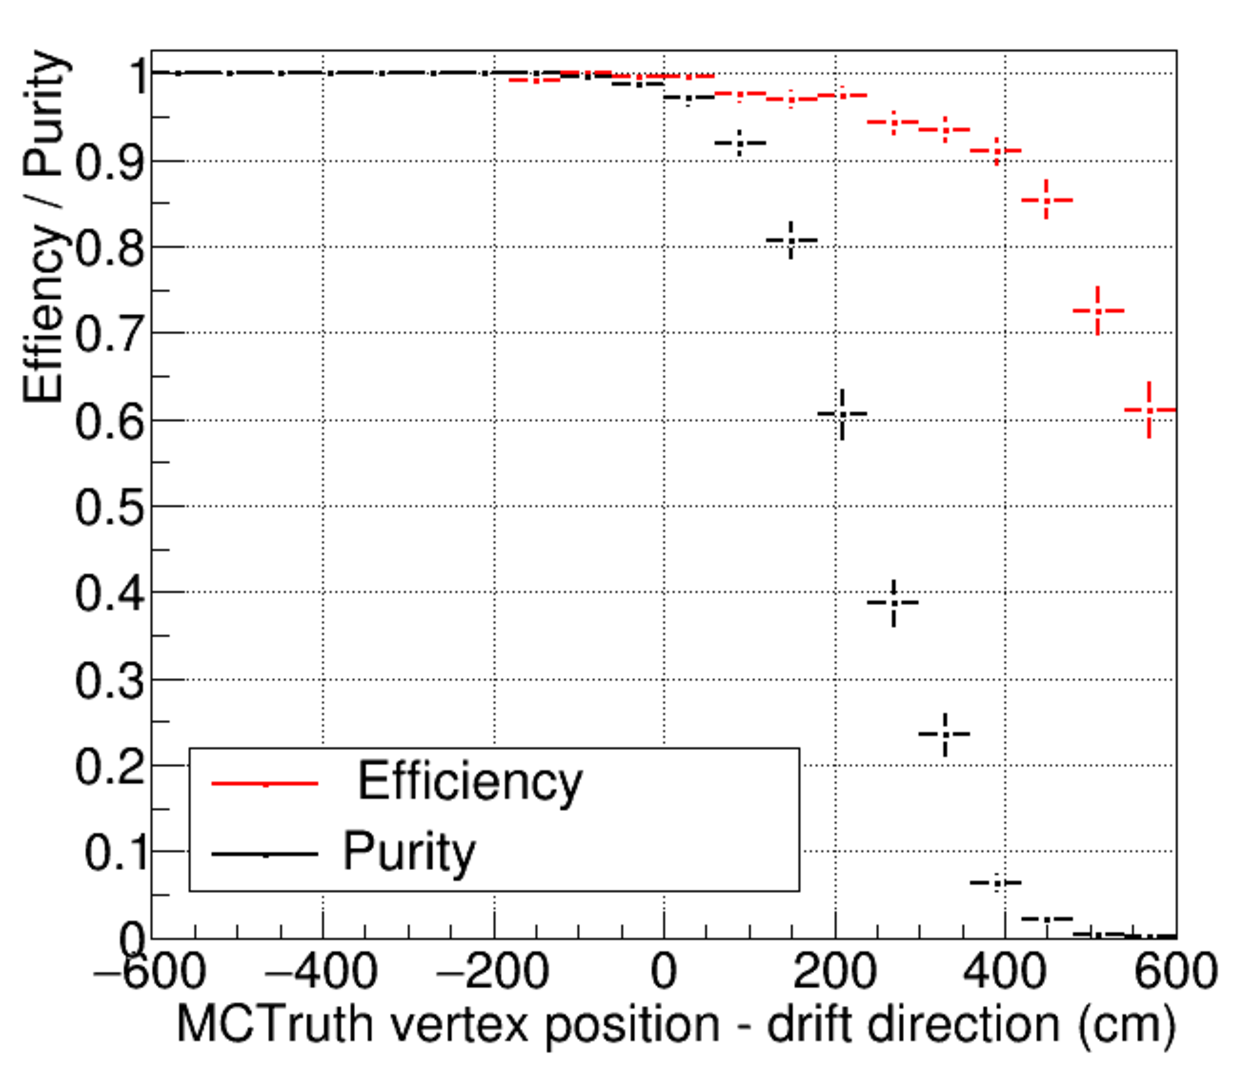
\includegraphics[width=0.5\textwidth]{graphics/dppd_ndk_efficiency.pdf}
    \end{dunefigure}

\fixme{Update NDK plots to include three cases: no foils, full foils, half foils.}

%%%%%%%%%%%%%%%%%%%%%%%%%%%%%%%%%%%%%%%%%%%%%%%%%%%%%%%%%%%%%%%%%%%%

\subsection{Supernova Burst Triggering}
\label{subsec:dp-pds-performance_trigger}

We have also studied the capability of the \dword{dp} \dshort{pds} to trigger on a SN burst occurring in our galactic neighbourhood. As described in Sec.~\ref{sec:dp-pds-requirements}, this is one of the primary goals of the system. To this end, SN \nue \dword{cc} interactions have been generated with MARLEY \cite{marley}. In \dword{dune}, a real-time algorithm is expected to provide trigger primitives by searching for \dshort{pmt} hits and optical clusters, where the latter combine several hits together based on their time/spatial information. Compared to the NDK case, the reconstructed optical signals are much weaker, since the typical deposited energies per SN neutrino interaction are of order \SI{20}{\MeV}. The online clustering process is similar to the offline cluster reconstruction discussed in Sec.~\ref{subsec:dp-pds-performance_t0}, albeit with some differences related to the lack of trigger information and detailed event reconstruction at this stage:
%
\begin{itemize}
\item Real-time optical clusters are required to have a minimum hit multiplicity to suppress clusters induced by radiological activity or \dword{pmt} dark counts. The higher the hit multiplicity, the lower the background cluster rate.
\item \dword{pds} spatial information is only used to group hits into separate clusters,  not to match \dword{pds} clusters with \dword{tpc} tracks in the plane perpendicular to the drift, as done in Sec.~\ref{subsec:dp-pds-performance_t0}.
\item Real-time optical clusters have to be continuously reconstructed, while in Sec.~\ref{subsec:dp-pds-performance_t0} only the \SI{7.5}{\milli\s} period preceding a charge-based trigger signal, corresponding to the maximum drift time, is considered.
\end{itemize}
%
In this case, the optimal real-time cluster reconstruction parameters, including a minimum hit multiplicity per cluster requirement, are found to yield a \SI{0.05}{\Hz} radiological background cluster rate for a SN \nue \dword{cc} signal cluster efficiency of \SI{7.7}{\%}. Once the optimal cluster parameters are found, the computation of the \dshort{pds}-based trigger efficiency for SN bursts as a function of SN distance is performed as follows:

\begin{itemize}
\item In a first step, the minimum number of reconstructed clusters required in a \SI{2.5}{\s} time window in order to issue a trigger is found\footnote{A \SI{2.5}{\s} time window was found to be optimal and is assumed throughout this section.}. The minimum cluster multiplicity is set by the requirement of one fake trigger per month at most (see Sec.~\ref{sec:dp-pds-requirements}), and by the radiological background cluster rate. The higher the background cluster rate, the higher the minimum cluster multiplicity has to be in order to meet the $<$\num{1}/month fake trigger rate requirement. As mentioned above, the clustering optimization procedure yields a background cluster rate of \SI{0.05}{\Hz}, or \num{0.125} clusters per \SI{2.5}{\s} window, on average. For such a background rate level, a minimum cluster multiplicity of $\ge$\num{4} per \SI{2.5}{\s} time window is required for a $<$\num{1}/month fake trigger rate.
%
\item In a second step, and given the cluster parameters and the minimum cluster multiplicity defined in the first step, the SN burst triggering efficiency as a function of the number of SNB interactions is computed. For a \SI{7.7}{\%} average efficiency of reconstructing single SN \nue interactions with the \dshort{pds}, and a minimum cluster multiplicity of \num{5} in order to issue a trigger, about \num{5}/\num{0.077}$\simeq$ \num{60} interactions have to occur in the FD module and within \SI{2.5}{\s} in order to obtain a non-negligible trigger efficiency. 
%
\item In a third and final step, the SN burst triggering efficiency as a function of SN distance is obtained. We use the theoretical assumptions shown in Fig.~\ref{fig:dppd_snbassumptions} to extract the number of SN neutrino interactions in a \SI{2.5}{\s} time window and in one \dword{dp} \dword{fd} module as a function of SN distance. The left panel of Fig.~\ref{fig:dppd_snbassumptions} shows the time-integrated expected number of SN neutrino interactions as a function of distance, while the right panel in Fig.~\ref{fig:dppd_snbassumptions} shows the assumed time profile of the burst during the first \SI{10}{\s}. Several hundred SN neutrino interactions are expected in one DP FD module for a \SI{10}{\kilo\parsec} distant SN, and about half of them are expected within the first \SI{2.5}{\s}. Given our earlier estimate that about \num{60} interactions are expected to be sufficient for a non-negligible trigger efficiency, it is clear that the \dshort{pds} should provide a high SN burst trigger efficiency for a SN at a \SI{10}{\kilo\parsec} distance.
\end{itemize}

\begin{dunefigure}[SN burst triggering assumptions.]{fig:dppd_snbassumptions}
     {Left panel: expected number of SN \nue \dshort{cc} interactions in one \dpactivelarmass active mass DP module as a function of SN distance. The different green lines indicate different SN burst models. Right panel: expected time profile of the SN burst.}
    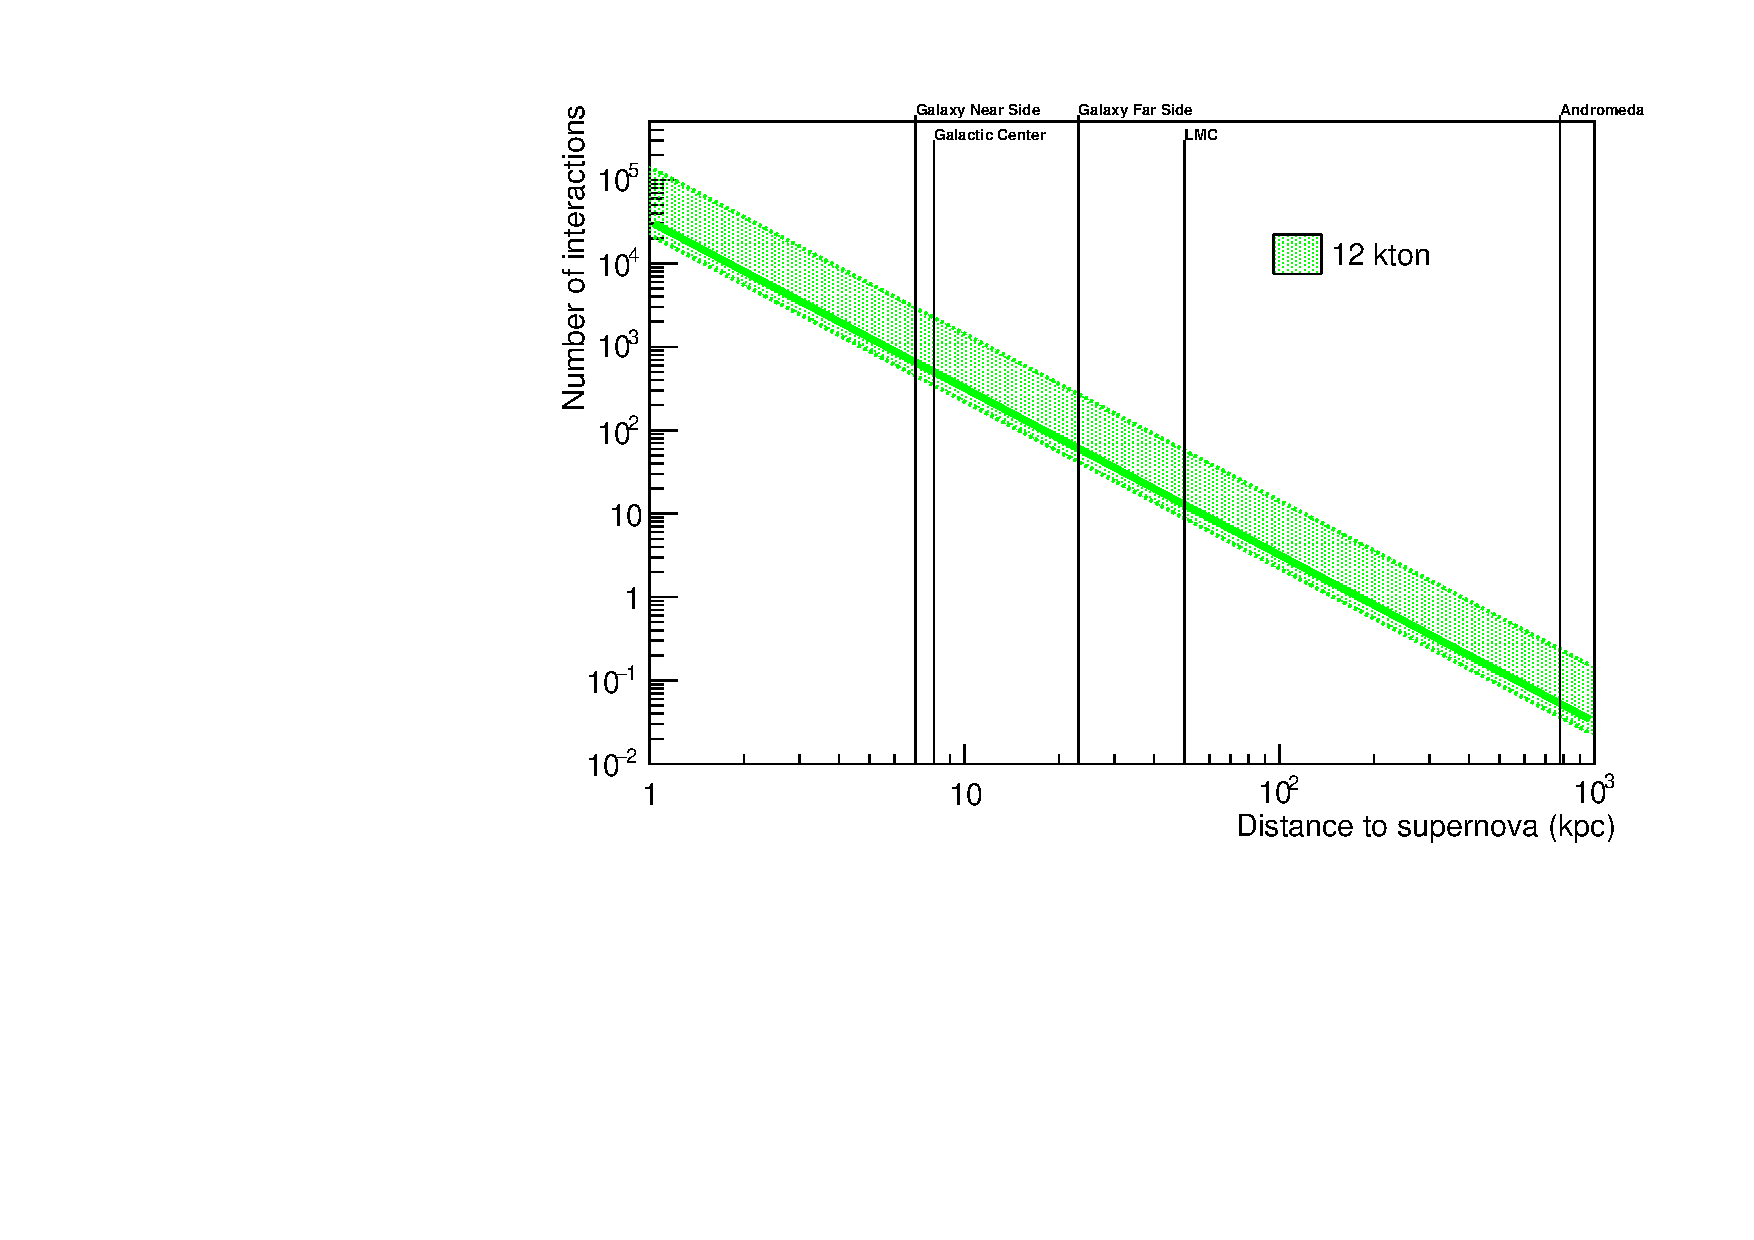
\includegraphics[width=0.49\textwidth]{graphics/dppd_events_vs_sndistance.pdf} \hfill
    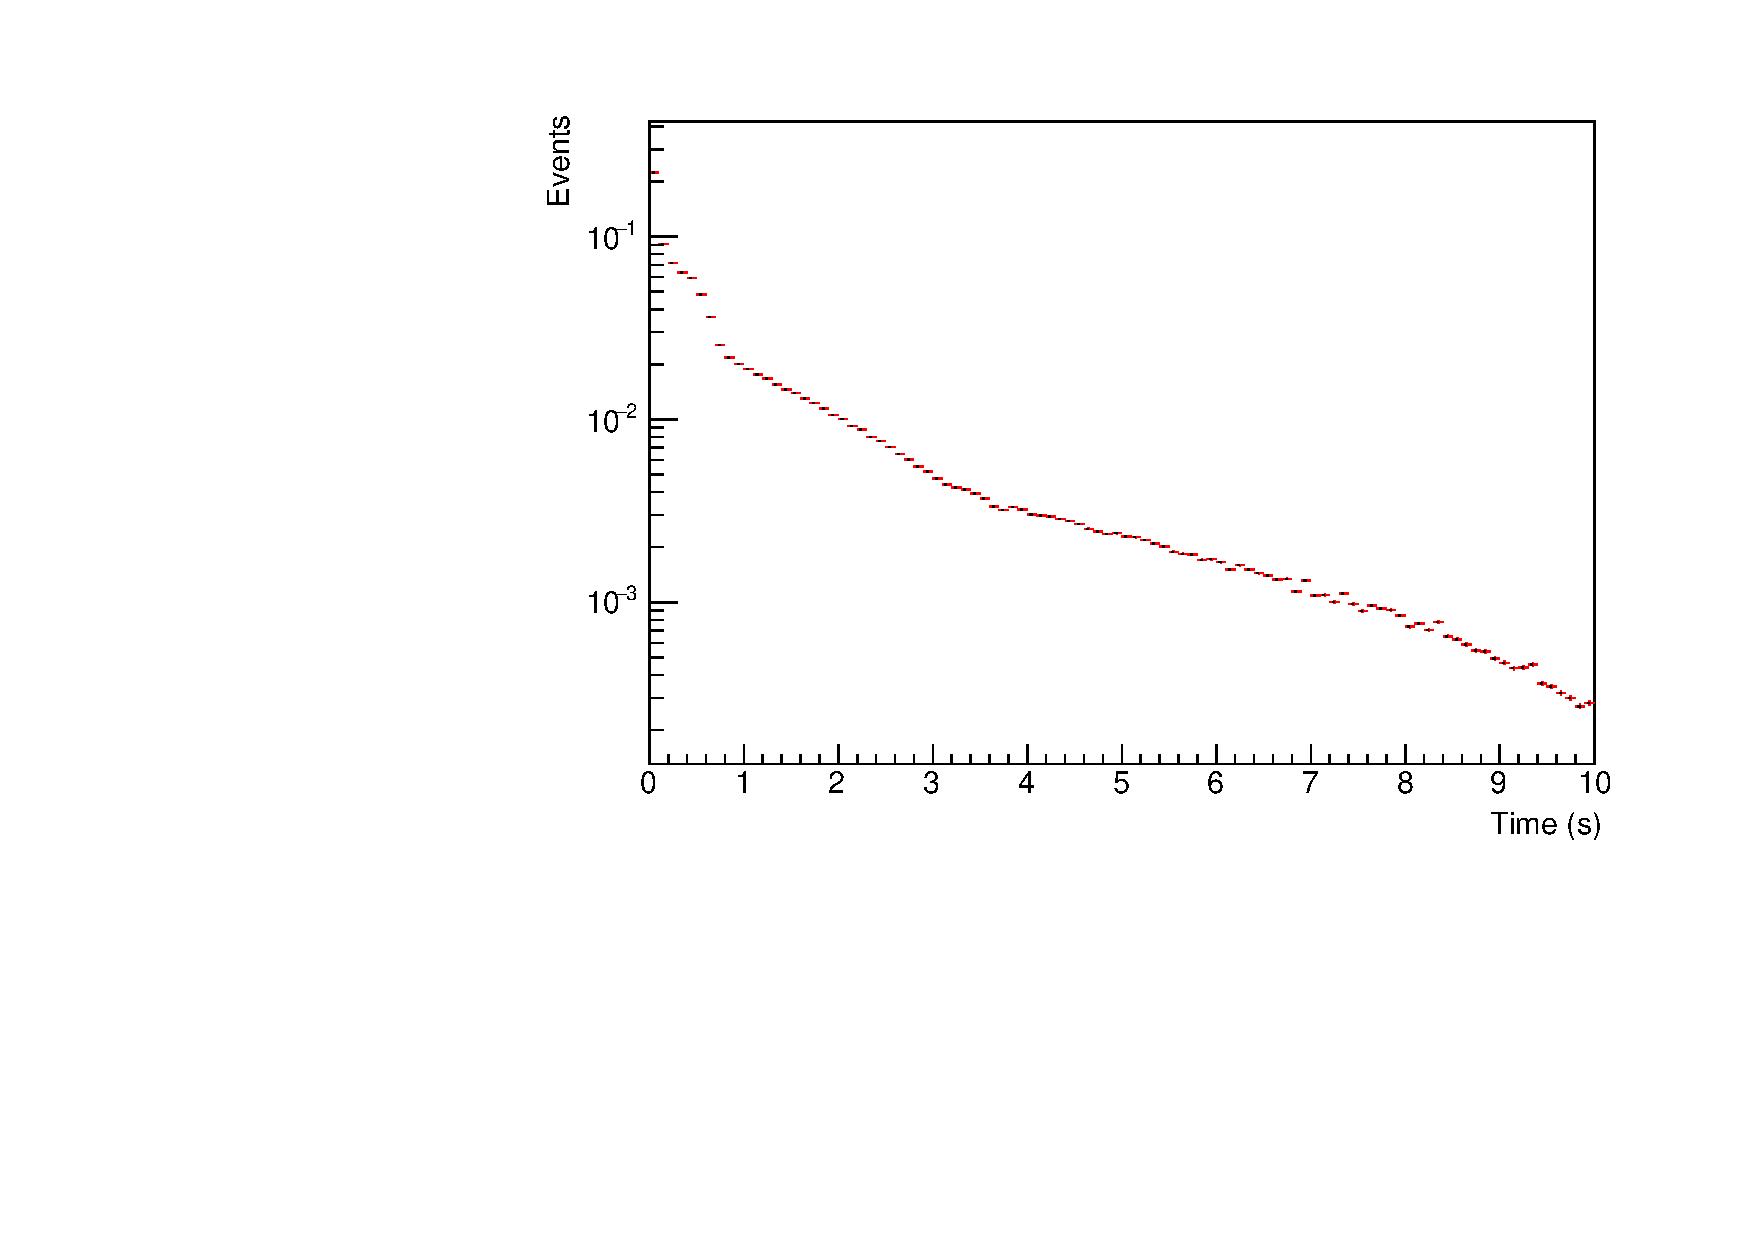
\includegraphics[width=0.49\textwidth]{graphics/dppd_sntime_profile.pdf} 
    \end{dunefigure}

The SN burst triggering efficiency, computed following the procedure described above and as a function of SN distance, is shown in Fig.~\ref{fig:dppd_snbefficiency_vs_sndistance}. The figure shows how the SN burst triggering efficiency is affected by different choices of the cluster reconstruction parameters. The best trigger efficiency is found for the cluster parameters yielding the lowest background cluster rate, \SI{0.05}{\Hz}. In this case, a trigger efficiency in excess of \num{90}\% is obtained up to SN distances of about \SI{20}{\kilo\parsec}. Therefore, the \dshort{pds} is expected to yield a highly efficient trigger for SN bursts occurring anywhere in the Milky Way. These expectations are based on a \dshort{pds} simulation without \dshort{wls} reflector foils, corresponding to an average light yield of \SI{3}{PEs/\MeV}. For this reason, Table~\ref{tab:specs:just:DP-PDS} quotes \SI{>3}{PEs/\MeV} as the average light yield requirement.

\begin{dunefigure}[SN burst triggering efficiency.]{fig:dppd_snbefficiency_vs_sndistance}
     {SN burst triggering efficiency using \dword{dp} \dshort{pds} information as a function of SN distance. Different curves indicate different choices of the optical cluster reconstruction parameters, resulting in different SN \nue signal detection efficiencies (DE) and radiological background rates (BGR).}
    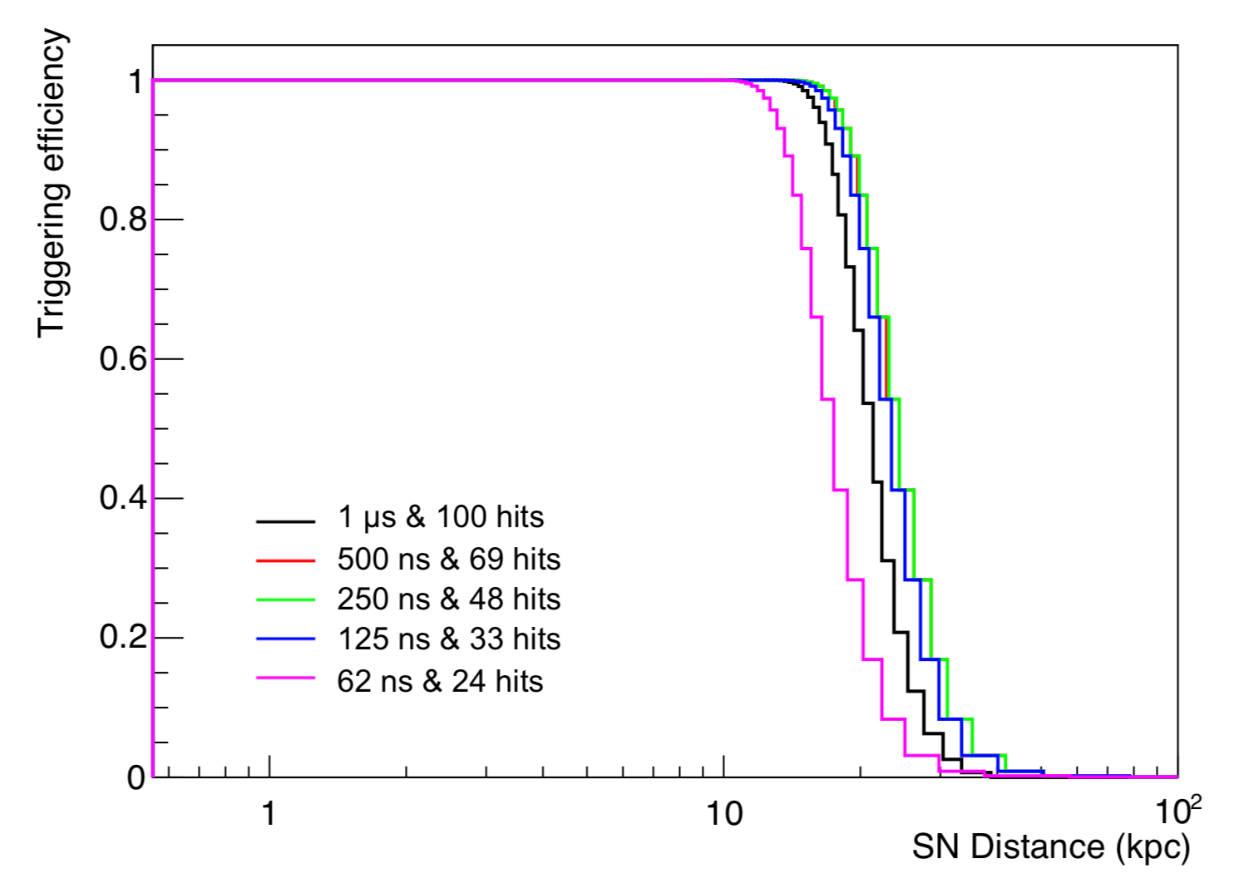
\includegraphics[width=0.6\textwidth]{graphics/dppd_snbefficiency_vs_sndistance.pdf}
    \end{dunefigure}

\fixme{Update SNB plots to include three cases: no foils, full foils, half foils.}

%%%%%%%%%%%%%%%%%%%%%%%%%%%%%%%%%%%%%%%%%%%%%%%%%%%%%%%%%%%%%%%%%%%%

\subsection{Event Energy Reconstruction}
\label{subsec:dp-pds-performance_calorimetry}

In addition to timing and triggering information, the photon detector system can also provide event energy information via the intensity of the reconstructed optical flashes. We focus in this section on beam neutrino interactions generated via the \dshort{genie} event generator \cite{Andreopoulos:2009rq}, as motivated in Sec.~\ref{subsec:dp-pds-requirements_requirements}.

A first requirement for a competitive energy reconstruction performance with the \dword{pds} is that optical hit saturation effects are kept to a manageable level by the \dword{pds} and associated readout electronics. Figure~\ref{fig:dppd_saturation} shows the expected average hit charge and average hit amplitude as a function of drift position of the neutrino interaction vertex, for \SI{3}{\GeV} beam \nue \dshort{cc} interactions. For each event, the average is computed by considering hit \dshort{pds} channels only, that is \dwords{pmt} detecting a charge of at least \SI{1}{PE}. The average hit charge per event is of order \SIrange{50}{300}{} for \SI{3}{\GeV} beam \nue \dshort{cc} interactions throughout the \dword{tpc} active volume. The average charge is expressed in PEs, while the average amplitude in PEs per \SI{4}{\nano\s} time bin. This time bin width is comparable with the \SI{6}{\nano\s} timescale characteristic of the prompt scintillation light in \dshort{lar}. For events near the cathode plane, about \SI{300}{PEs} per hit channel are detected, corresponding to a maximum amplitude over \SI{4}{\nano\s} of about \SI{50}{PEs}. The factor of 6 difference between average charge and average amplitude is due to the fact that only \SI{23}{\%} of the scintillation light is prompt, and (to a smaller extent) to additional time smearing introduced by light propagation to the same \dword{pmt} from different \dshort{lar} voxels containing energy deposits. From these plots, we conclude that the \dshort{pds} signal readout should withstand signal amplitudes of at least \SI{100}{PEs} over \SI{6}{\nano\s} to mitigate saturation effects, as stated in Table~\ref{tab:specs:just:DP-PDS}

\begin{dunefigure}[Average charge and amplitude per hit channel in beam neutrino interactions.]{fig:dppd_saturation}
{Expected average hit charge (left panel, in PEs) and average hit amplitude (right panel, in PEs per \SI{4}{\nano\s} time bin) as a function of event drift position, for \SI{3}{\GeV} beam \nue \dshort{cc} interactions. The scatter plots  contain one entry per event, and the average is made over hit \dshort{pds} channels only.}
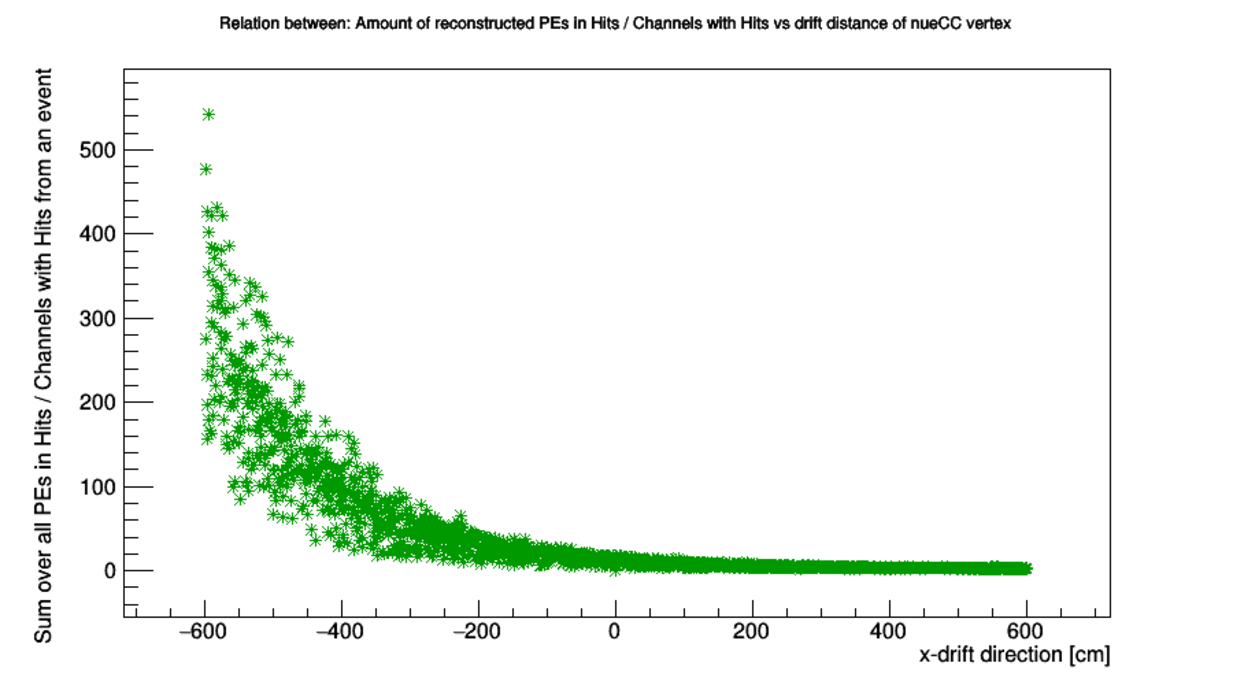
\includegraphics[trim={0cm 0cm 0cm 1.cm}, clip, width=0.49\textwidth]{graphics/dppd_avg_charge_per_channel.pdf} \hfill
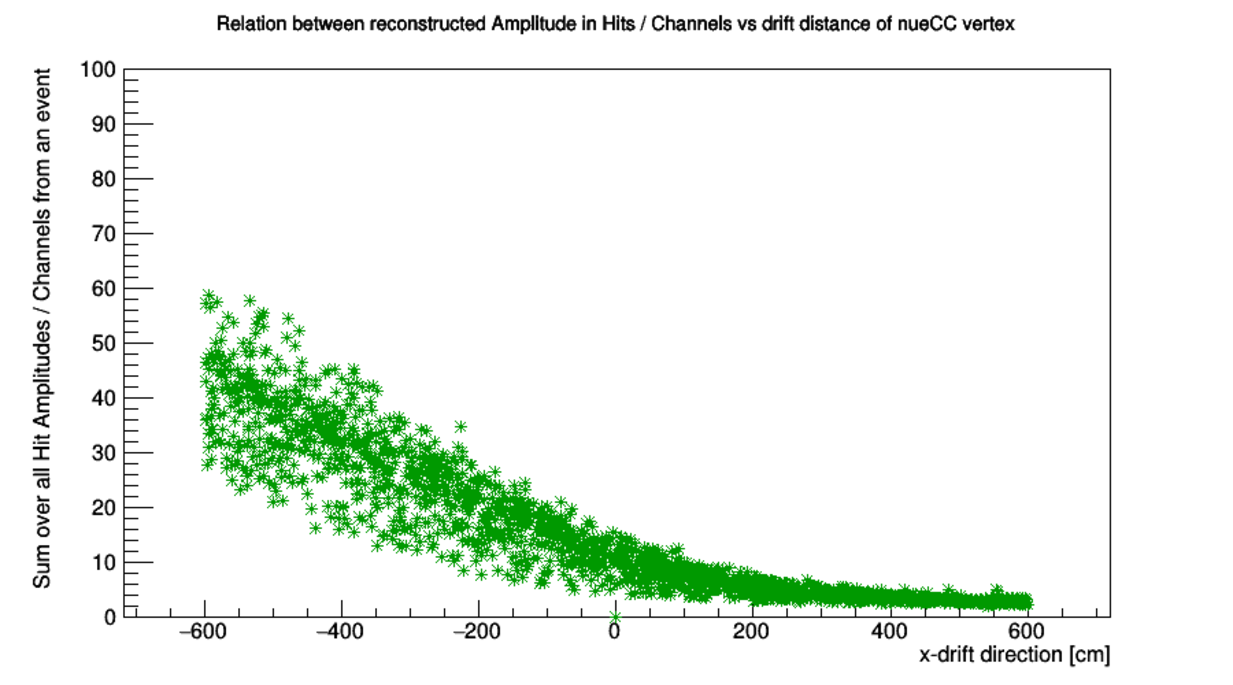
\includegraphics[trim={0cm 0cm 0cm 1.cm}, clip, width=0.49\textwidth]{graphics/dppd_avg_amplitude_per_channel.pdf}
\end{dunefigure}


\fixme{Add full study of PDS-based energy reconstruction performance, using simulated beam \nue \dword{cc} interactions.} 